\chapter{Przegląd literatury}
\section{Wytyczne postępowania klinicznego}
Wytyczne postępowania klinicznego to przygotowany w sposób systematyczny zestaw zaleceń odnośnie postępowania (diagnozowania, planowania terapii, realizacji procesu terapeutycznego) w specyficznych warunkach, np. dla określonego schorzenia czy też urazu \cite{Latoszek-Berendsen} (dla uproszczenia, w dalszej części tekstu będzie mowa o specyficznych chorobach).

Pierwsze wytyczne kliniczne zaczęły pojawiać się ponad 30 lat temu. Ich celem było ograniczenie zmienności w postępowaniu, jego ujednolicenie oraz optymalizacja pod względem wykorzystywanych kosztów i innych zasobów. Początkowo wytyczne były przygotowywane dla personelu pomocniczego (np. dla pielęgniarek), dopiero potem do grona potencjalnych „użytkowników” włączono lekarzy (było to związane z obawami środowiska lekarskiego przed tzw. \textit{cookbook medicine}, czyli medycyną według przepisu) \cite{Latoszek-Berendsen}. Praktyczna akceptacja wytycznych jest wciąż ograniczona -- o przyczynach takiego stanu rzeczy będzie mowa w dalszej części rozdziału.\\*
Do reprezentowania wytycznych wykorzystywane są dwa modele:
\begin{enumerate}
\item model tekstowy, w którym wytyczne są prezentowane w postaci dokumentu tekstowego. Aby ułatwić jego przeglądanie lub przeszukiwanie, tekst jest wzbogacany o dodatkowe znaczniki (standard GEM) nadające semantykę wybranym jego fragmentom,
\item model sieci zadań (ang. \textit{task network model}), w którym wytyczne są reprezentowane jako graf skierowany. Wierzchołki w grafie odpowiadają podstawowym krokom w wytycznych -- zebraniu danych, podjęciu decyzji, czy też wykonaniu akcji klinicznej. Krawędzie (łuki) wskazują natomiast na zależności kolejnościowe między poszczególnymi krokami. Ten właśnie model stanowi podstawę wielu formalnych reprezentacji wytycznych (np. GLIF3, PROforma, GLARE, SAGE).
\end{enumerate}

W ciągu ostatnich lat rośnie popularność reprezentacji wytycznych wykorzystujących sieci zadań ze względu na możliwość ich osadzenia w systemach komputerowych -- mówi się nawet o nowej klasie wytycznych, czyli o wytycznych interpretowanych komputerowo (ang. \textit{computer interpretable guidelines}, CIG). Dzięki temu można budować SWDK, które pozwalają na połączenie wytycznych z danymi dostępnymi w wersji elektronicznej automatyzując tym samym proces opracowywania sugestii diagnostycznych i terapeutycznych dla konkretnego pacjenta. Takie „skomputeryzowane” wytyczne są przedmiotem intensywnych badań, które można podzielić na następujące kategorie:
\begin{enumerate}
\item modelowanie i reprezentacja wytycznych,
\item pozyskiwanie i definiowanie wytycznych,
\item integracja z systemami szpitalnymi (zwłaszcza z elektroniczną kartą pacjenta),
\item walidacja i weryfikacja wytycznych,
\item wykonywanie wytycznych,
\item obsługa sytuacji wyjątkowych,
\item utrzymanie i „pielęgnacja” wytycznych,
\item współdzielenie wytycznych.
\end{enumerate}

Niniejsza praca magisterska dotyczy obsługi sytuacji wyjątkowych związanych z konfliktami, które mogą pojawić się podczas jednoczesnego wykonania wielu wytycznych dla jednego pacjenta. Odpowiada ona w ten sposób na wyzwanie związane z jednym z głównych ograniczeń wytycznych, tzn. skupieniem się na jednym specyficznym problemie. Ograniczenie to jest jedną z istotnych przyczyn słabego praktycznego przyjęcia i wykorzystania wytycznych i jest też jednym z głównych wyzwań dla SWDK \cite{Sittig08}.

\section{Wykrywanie i usuwanie konfliktów w wytycznych}

\subsection{Programowanie logiczne z ograniczeniami}

W pracy \cite{SzWilk2} przedstawiono podejście wykorzystujące programowanie logiczne z ograniczeniami (ang. \textit{constraint logic programming}, CLP -- szczegółowy opis w rozdziale \ref{sec:clp}) do wykrywania i usuwania konfliktów dla pary wytycznych. Podejście to zakłada, że wytyczne prezentowane są w postaci grafu akcji (ang. \textit{actionable graph}). Graf akcji jest uproszczoną siecią zadań -- jest grafem skierowanym, w którym występują trzy typy węzłów:
\begin{itemize}
\item \textit{węzeł kontekstu} wskazujący na chorobę, której dotyczą wytyczne,
\item \textit{węzeł akcji} opisujący akcję kliniczną, jaką należy wykonać,
\item \textit{węzeł decyzyjny} opisujący decyzję i możliwe opcje.
\end{itemize}

W grafie akcji zrezygnowano z jawnego węzła odpowiadającego pozyskaniu danych i założono, że dane są pozyskiwane w węzłach decyzyjnych (np. poprzez zadanie odpowiedniego pytania lekarzowi). Przykład grafu akcji (rozszerzonego o możliwość zawierania ścieżek równoległych) przedstawiono na rys. \ref{fig:sciezki_rownolegle}.

Grafy akcji są automatycznie tłumaczone na modele logiczne i automatycznie przetwarzane. Podejście to wykorzystuje dodatkową wiedzę dziedzinową (nie pojawiającą się jawnie w wytycznych) reprezentowaną w formie operatorów interakcji (ang. \textit{interaction operators}) oraz modyfikacji (ang. \textit{revision operators}). Operator interakcji reprezentuje możliwy konflikt (zazwyczaj lek-lek lub lek-choroba), natomiast operator modyfikacji opisuje natomiast zmiany, jakie należy wprowadzić do modeli logicznych, aby konflikt usunąć. Oba operatory przedstawione są w formie wyrażeń logicznych.
\\*
Schemat działania podejścia przedstawiono na rys. \ref{fig:algorytm-clp}. Obejmuje on dwie fazy:
\begin{enumerate}
\item wyszukiwanie bezpośrednich konfliktów między wytycznymi (tzn. konfliktów, gdzie jedne wytyczne zalecają akcję \textit{A}, a drugie zabraniają tej akcji -- konflikty takie objawiają się jako niespójne wartości zmiennych współdzielonych przez modele logiczne) i ich usunięcie za pomocą operatorów modyfikacji,
\item wyszukanie pośrednich konfliktów (opisanych za pomocą operatorów interakcji) i ich usunięcie za pomocą operatorów modyfikacji.
\end{enumerate}

\begin{figure}[H]
\begin{center}
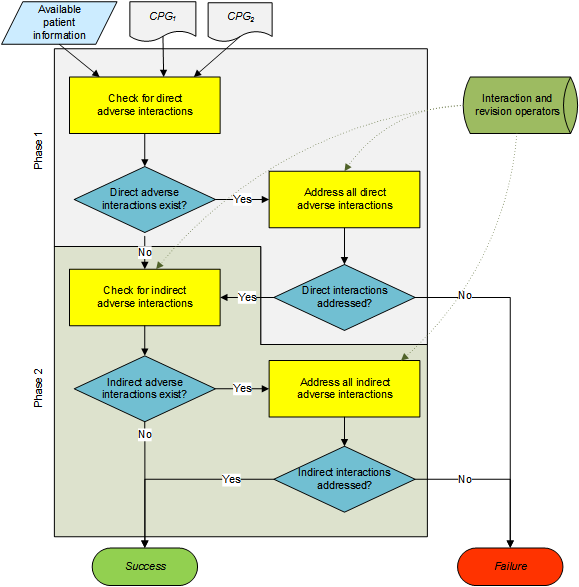
\includegraphics[scale=0.6]{img/algorytm-clp.png}
\end{center}
\caption{Schemat działania podejścia wykorzystującego CLP \cite{SzWilk2}}
\label{fig:algorytm-clp}
\end{figure}

Podczas obu faz działania na podstawie modeli logicznych tworzone są programy CLP, które są następnie wykonywane/rozwiązywane. Uzyskane rozwiązanie wskazuje na terapię rozumianą jako ścieżki w grafach akcji, jakie należy przejść podczas leczenia pacjenta. Rozwiązanie uzyskane w ostatniej fazie jest ostateczną terapią prezentowaną lekarzowi.

Opisane podejście posiada kilka wad -- jest ograniczone tylko do dwóch wytycznych, nie pozwala na uwzględnianie dawek leków oraz pozwala tylko na proste zmiany (jedna operacja) wprowadzane przez operatory modyfikacji. Rozszerzenia zaproponowane w ramach tej pracy magisterskiej usuwają te wady.



\subsection{Logika pierwszego rzędu}

W pracy \cite{SzWilk} przedstawiono rozwinięcie opisanego powyżej podejścia, w którym CLP zastąpiono przez logikę pierwszego rzędu (ang. \textit{first-order logic}, FOL). Dzięki temu uzyskano znacznie bogatszą semantykę uwzględniającą zależności kolejnościowe między krokami, dawki leków, czy też złożone operacje modyfikacji wytycznych. Zmodyfikowano również algorytm wykrywania i usuwania konfliktów, aby uwzględniał wiele wytycznych. Podobnie jak poprzednio, wytyczne są podane w formie grafów akcji, a wiedza dziedzinowa w formie operatorów interakcji i rewizji.

Minusem tego podejścia są bardziej złożone modele reprezentujące wytyczne (konieczne jest definiowanie reguł kontrolujących proces wnioskowania) oraz konieczność stosowania bardziej złożonych narzędzi (m.in. systemów do dowodzenia twierdzeń). Z uwagi na te komplikacje, w pracy magisterskiej skupiono się na wcześniejszym podejściu z CLP.



\subsection{Podejście wykorzystujące paradygmat mieszanej inicjatywy}

Paradygmat mieszanej inicjatywy (ang. \textit{mixed initiative paradigm}) polega na tym, że podczas rozwiązywania problemu użytkownik współpracuje z systemem komputerowym, a zatem nie ma tutaj działania w pełni automatycznego. Paradygmat ten został wykorzystany w pracy \cite{Piovesan} do wykrywania i usuwania konfliktów między wytycznymi. Podobnie jak we wcześniej opisywanych podejściach, również tutaj wytyczne reprezentowane są w postaci grafu (formalizm GLARE) składającego się z węzłów będących akcjami (dopuszcza sie zarówno akcje atomowe, jak i złożone, czyli plany) i krawędzi modelujących relacje między akcjami. Natomiast wiedza dziedzinowa o możliwych interakcjach reprezentowana jest w formie ontologii (wraz z towarzyszącą bazą wiedzy), która wykorzystuje istniejące terminologie i klasyfikacje medyczne, np. SNOMED CT dla pojęć medycznych i ACT dla leków.
  
Opisywane podejście stosuje dwie grupy metod do unikania i rozwiązywania zidentyfikowanych konfliktów:
\begin{enumerate}
	\item unikanie konfliktów
	\begin{itemize}
		\item wybieranie bezpiecznej alternatywy, tzn. takiej ścieżki w grafie, w której konflikt nie występuje,
		\item czasowe unikanie konfliktu, np. poprzez odpowiednie planowanie działań,
	\end{itemize}
	\item naprawienie konfliktów
	\begin{itemize}
		\item modyfikacja dawek leków,
		\item monitorowanie efektów (tutaj dopuszcza się mniej poważne konflikty i na bieżąco monitoruje ich następstwa),
		\item osłabianie interakcji poprzez rozszerzanie zaleceń o dodatkowe akcje.
	\end{itemize}
\end{enumerate}

Do przetwarzania wytycznych wykorzystywane jest wsteczne przeszukiwanie grafów reprezentujących wytyczne (np. w celu szukania bezpiecznych ścieżek), planowanie bazujące na celach (np. w celu monitorowania efektów konfliktowych akcji) oraz wnioskowanie temporalne (w celu unikania konfliktów lub planowania razem wzmacniających się akcji). Podejście to uwzględnia również pozytywne interakcje i pozwala na takie planowanie akcji, aby dochodziło do pożądanego wzmacniania ich efektów oraz wykrywa dublujące się akcje (np. podane tego samego leku pojawiające się w kilku zaleceniach).

Jak już wspomniano, podejście to nie jest automatyczne -- lekarz wskazuje na odpowiedni sposób postępowania, a system stara się go zrealizować. Poza tym podejście to wymaga rozbudowanej i szczegółowej wiedzy dziedzinowej  podanej w formie ontologii.



